%! TeX program = lualatex
\documentclass[main]{subfiles}

\begin{document}

\title[AutoML: BO]{Noisy Bayesian Optimization}
\subtitle{Surrogates, Acquisitions, and Final Best Under Noise}
\author[Bernd Bischl]{Bernd Bischl}
\date{}

\titlebackground*{images/AutoML_HPO_bayesian3.jpg}

    \maketitle


\begin{frame}[t]{Noisy Evaluations}
  \begin{itemize}
    \item So far we assumed noise-free evaluations of $\cost(\conf)$
    \item In practice we only observe a noisy read-out
        $$y = \cost(\conf) + \epsilon, \quad \epsilon \sim \normaldist(0, \noisevar)$$    
    \item Sources in HPO: resampling, stochastic learners
    \item Also common in computer experiments
    \item NB: We usually want inference on $\cost(\conf)$ (true signal) not $y(\conf)$
  \end{itemize}
  \vfill
  \begin{center}
    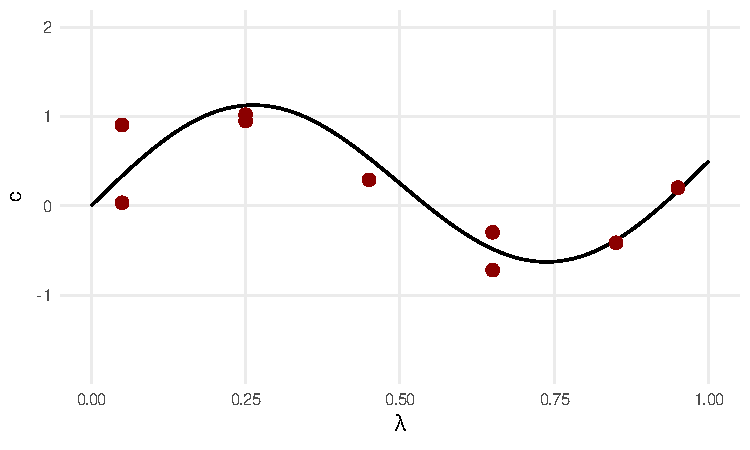
\includegraphics[width=.45\textwidth, height=2.5cm, keepaspectratio]{images/07_noisy_data.pdf}
  \end{center}
\end{frame}


\begin{frame}[t]{Noise-Aware Surrogate: Nugget GP}
  % \textbf{Issue:} an interpolating GP forces $\sh^2(\confI{i}) = 0$ at design points -- under noise the posterior should stay uncertain.
  \begin{columns}[onlytextwidth,T]
    \column{.55\textwidth}
    \begin{itemize}
      \item Add nugget $\noisevar \bm{I}$ to the kernel matrix:
        $$\surro(\conf) = k_*^T (\bm{K} + \noisevar \bm{I})^{-1} \yv$$
        $$\sh^2(\conf) = k_{**} - k_*^T (\bm{K} + \noisevar \bm{I})^{-1} k_*$$
      \item Posterior \textbf{smooths} through the data instead of interpolating
      \item $\sh^2(\confI{i}) > 0$ even at design points
      \item $\noisevar$ learned via max. likelihood alongside kernel parameters
      \item We covered this before
    \end{itemize}
    \column{.45\textwidth}
    \begin{center}
      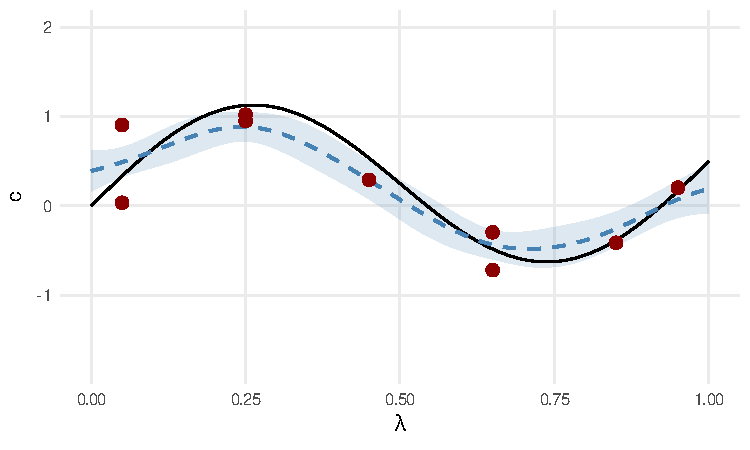
\includegraphics[width=\textwidth]{images/07_noisy_nugget.pdf}
    \end{center}
  \end{columns}
\end{frame}


\begin{frame}[t]{Noise-Aware Acquisition: AEI and NEI}
  \small
  \begin{itemize}
    \item PI / EI use $\cmin = \min_i y_i$, but this is noisy $\leadsto$ lucky outliers dominate
    \item \textbf{Plug-in EI:} replace unknown $\cmin$ with an \textbf{effective best}
    $\cmin^* = \min_i \surro(\confI{i}) + \beta\, \sh(\confI{i})$; risk-aversion $\beta \ge 0$ down-weights uncertain points
    \item \textbf{Augmented EI}~\liturl{Huang et al. 2006}{https://link.springer.com/article/10.1007/s10898-005-2454-3}: plug-in EI times a diminishing-returns penalty
    $$\acq_{\text{AEI}}(\conf) = \acq_{\text{EI}_{\cmin^*}}(\conf) \cdot \left(1 - \frac{\sqrt{\noisevar}}{\sqrt{\sh^2(\conf) + \noisevar}}\right)$$
    \item Penalty shrinks acquisition where the GP is already certain $\leadsto$ redirects budget to replication and exploration; recovers standard EI as $\noisevar \to 0$
    \item \textbf{Noisy EI (NEI)}~\liturl{Letham et al. 2019}{https://projecteuclid.org/journals/bayesian-analysis/volume-14/issue-2/Constrained-Bayesian-Optimization-with-Noisy-Experiments/10.1214/18-BA1110.full}: MC-integrate EI over sampled posterior fantasy functions from the GP -- no plug-in needed
    \item \textbf{LCB needs no patch:} no $\cmin$ in the formula, so a nugget GP alone suffices
  \end{itemize}
\end{frame}


\begin{frame}[t]{Which Point to Return?}
  Choice of incumbent rule benchmarked in~\liturl{Picheny et al. 2013}{https://link.springer.com/article/10.1007/s00158-013-0919-4}
  \begin{itemize}
    \item Empirical best $\argmin_i y_i$: noisy, vulnerable to lucky outliers
    \item \textbf{Model-based:} $\argmin_i \surro(\confI{i})$
    \item \textbf{Risk-averse:} $\argmin_i \surro(\confI{i}) + \beta\, \sh(\confI{i})$ (Huang's plug-in)
    \item \textbf{Replication:} re-evaluate current best to sharpen its estimate
    \item \textbf{Domain-wide:} $\argmin_{\conf \in \pcs} \surro(\conf)$ -- trust only if GP is well-calibrated
  \end{itemize}
\end{frame}


\begin{frame}[t]{Summary}
  \begin{itemize}
    \item \textbf{Surrogate:} switch to a nugget GP (regression mode)
    \item \textbf{Acquisition:} we covered plugins, AEI, NEI, and LCB
    \item \textbf{Final best:} model-based or risk-averse incumbent
  \end{itemize}
\end{frame}


\end{document}
